\documentclass[12pt, titlepage]{article}

\usepackage{fullpage}
\usepackage[round]{natbib}
\usepackage{multirow}
\usepackage{booktabs}
\usepackage{tabularx}
\usepackage{graphicx}
\usepackage{float}
\usepackage{hyperref}
\hypersetup{
    colorlinks,
    citecolor=black,
    filecolor=black,
    linkcolor=red,
    urlcolor=blue
}
\usepackage[round]{natbib}

\newcounter{acnum}
\newcommand{\actheacnum}{AC\theacnum}
\newcommand{\acref}[1]{AC\ref{#1}}

\newcounter{ucnum}
\newcommand{\uctheucnum}{UC\theucnum}
\newcommand{\uref}[1]{UC\ref{#1}}

\newcounter{mnum}
\newcommand{\mthemnum}{M\themnum}
\newcommand{\mref}[1]{M\ref{#1}}

\title{SE 3XA3: Module Internal Specification\\MAC Schedule Importer}

\author{Team 12, 0C
		\\ Cassandra Nicolak, nicolace
		\\ Michelle Leung, leungm16
		\\ Winnie Liang, liangw15
}

\date{\today}

%\input{../../Comments}

\begin{document}

\maketitle

\pagenumbering{roman}
\tableofcontents
\listoftables
\listoffigures

\begin{table}[bp]
\caption{\bf Revision History}
\begin{tabularx}{\textwidth}{p{3cm}p{2cm}X}
\toprule {\bf Date} & {\bf Version} & {\bf Notes}\\
\midrule
Date 1 & 1.0 & Notes\\
Date 2 & 1.1 & Notes\\
\bottomrule
\end{tabularx}
\end{table}

\newpage

\pagenumbering{arabic}

\section{Introduction}
\subsection{General Overview and Introduction}
This document provides a complete description of the module guide for the MAC Schedule Importer, a desktop application that imports the user's Mosaic schedule into their Google calendar.\\

The intended audience of this document includes the following: 

\begin{itemize}
\item Software Development/Design teams, including Team 0C: This document provides a method for designers and developers to
  check for the feasibility, correctness and consistency of their program. 
\item New team members and third party software development teams: This document can be a reference guide which enables developers that are unfamiliar with the project to easily comprehend the general system design and structure. 
\item Maintainers: The document can be used to locate specific modules for maintenance and the described module decomposition in the module guide allows a better understanding of the system when changes are made. %It is important for a maintainer to update the relevant sections of the document after changes have been made.
\end{itemize}

The module guide document is organized as follows:\\
\begin{itemize}
\item Section \ref{SecChange} lists the anticipated and unlikely changes of the software
requirements.
\item Section \ref{SecMH} summarizes the module decomposition that
was constructed according to the likely changes.
\item  Section \ref{SecConnection}
specifies the connections between the software requirements and the
modules.
\item Section \ref{SecMD} gives a detailed description of the
modules.
\item  Section \ref{SecTM} includes two traceability matrices. One checks
the completeness of the design against the requirements provided in the SRS. The
other shows the relation between anticipated changes and the modules.
\item Section
\ref{SecUse} describes the use relation between modules.
\end{itemize}

\subsection{Motivation and Design Choices}
For large software system designs, the decomposition into smaller components, such as modules and sub-modules, is a necessity for organization and structure. Moreover, modular decomposition enables future modifications to various system components without altering majority of the system. Hence, Team 0C followed the 'design for change' pattern for the MAC Schedule Importer project. For example: 
\begin{itemize}
    \item Components of the system that are anticipated to change are encapsulated into 'secrets'.
    \item Each module contains one secret.
    \item Other members of the system that requires data from a module can only acquire the information through public access methods that are defined in that module.
\end{itemize}

\section{Anticipated and Unlikely Changes} \label{SecChange}

\subsection{Anticipated Changes} \label{SecAchange}
Design for change was incorporated into the software design for MAC Schedule Importer.   The anticipated changes, which will ideally change only the secrets hidden in modules without affecting the whole project, are listed below.

\begin{description}
\item[\refstepcounter{acnum} \actheacnum \label{acParser}:] The format of Mosaic schedule.
\item[\refstepcounter{acnum} \actheacnum \label{acOS}:] The operating systems which the software interfaces.
\item[\refstepcounter{acnum} \actheacnum \label{achardware}:] The hardware on which the software is running.
\item[\refstepcounter{acnum} \actheacnum \label{acScrapy}:] The syntax and functions of Scrapy.
\item[\refstepcounter{acnum} \actheacnum \label{acGoogle}:] The Google Calendar layout.
\end{description}

\subsection{Unlikely Changes} \label{SecUchange}

The following design decisions are not intended to change as modifications to these decisions lead to multiple subsequent changes to the whole system.

\begin{description}
\item[\refstepcounter{ucnum} \uctheucnum \label{ucIO}:] Input/Output devices
  (Input: File, Output: Screen).
\item[\refstepcounter{ucnum} \uctheucnum \label{ucInput}:] There will always be
  a source of input data external to the software.
\item[\refstepcounter{ucnum} \uctheucnum \label{ucParse}:] The parsing algorithm.
\item[\refstepcounter{ucnum} \uctheucnum \label{ucGoal}:] The main purpose of the program - To import a Mosaic schedule into Google Calendar.
\end{description}

\section{Module Hierarchy} \label{SecMH}
The module hierarchy is an overview of the general structure and design for the module. In Table \ref{TblMH}, the modules are shown in a hierarchy decomposition according to their respective secrets. 
The models below are the 'leaves' of the hierarchy tree and will be implemented.

\begin{description}
\item [\refstepcounter{mnum} \mthemnum \label{mHH}:] *Hardware-Hiding Module
\item [\refstepcounter{mnum} \mthemnum \label{mpM}:] parseMosaic Module
\item [\refstepcounter{mnum} \mthemnum \label{mcv}:] convertor Module
\item [\refstepcounter{mnum} \mthemnum \label{mcn}:] connect Module
\item [\refstepcounter{mnum} \mthemnum \label{mgc}:] guiClient Module
\end{description}

*Note: The Hardware-Hiding Module is not implemented for this software-based project. Inclusion of this module is for formality purposes.

\begin{table}[h!]
\centering
\begin{tabular}{p{0.3\textwidth} p{0.6\textwidth}}
\toprule
\textbf{Level 1} & \textbf{Level 2}\\
\midrule

{Hardware-Hiding Module} & ~ \\
\midrule

\multirow{3}{0.3\textwidth}{Behaviour-Hiding Module} & convertor\\
& connector\\
& guiClient\\
\midrule

%{Software Decision Module} & ~ \\
\multirow{1}{0.3\textwidth}{Software Decision Module} & parseMosaic\\
%& guiClient\\
%& ?\\
\bottomrule

\end{tabular}
\caption{Module Hierarchy}
\label{TblMH}
\end{table}

\section{Connection Between Requirements and Design} \label{SecConnection}

The design of the MAC Schedule Importer is designed to satisfy the requirements developed in
the SRS document. During this stage, the system is decomposed into modules. The connection
between requirements and modules is listed in Table \ref{TblRT}. It is recommended to read Section \ref{SecMH} and Section \ref{SecMD} before reading Section \ref{SecTM}.\\

%The guiClient module is the user interface of the MAC Schedule Importer. The module satisfies the requirement of interacting with the user to display notifications of the inability to access the Mosaic schedule or Google calendar. Additionally, it satisfies the requirements of the authorization of accessing the user's Mosaic schedule and Google account as well as verifying the changes made to the user's Google Calendar before proceeding. Also, the guiClient module meets the requirements of tracking the importing process, a simple user interface and help option provided to guide the user through the navigation of the system.\\

%The connector module returns the results and displays the user's Mosaic schedule in their Google Calendar. It satisfies the requirement of importing the user's Mosaic schedule into Google Calendar. As well, it ensures that the security requirement that the application shall not store or upload user information is satisfied as the module discards the information once the user finishes using the system.\\

%The parseMosaic module retrieves the information from the user's Mosaic schedule and passes the data to the converter. The module sa


\section{Module Decomposition} \label{SecMD}

The modules of MAC Schedule Importer are decomposed according to the principle of ``information hiding''
proposed by David Parnas. Each module is comprised of \emph{Secrets}, \emph{Service}, and \emph{Implemented by}.  The \emph{Secrets} in a module is a noun. It is a statement of the hidden design decision for the module. The \emph{services} specifies what the module will accomplish without specifying what methods the module will use to accomplish it. The  \emph{Implemented By} title is a tentative idea for the implementing software of each module.
 %If the entry is \emph{OS}, this means that the module is provided by the operating system or by standard programming language libraries.  %Also indicate if the module will be implemented specifically for the software.

%Only the leaf modules in the hierarchy have to be implemented. If a dash (\emph{--}) is shown, this means that the module is not a leaf and will not have to be implemented. Whether or not this module is implemented depends on the programming language selected.

\subsection{Hardware Hiding Modules (\mref{mHH})}

\begin{description}
\item[Secrets:]The algorithm and data structure that are used to implement the virtual hardware.
\item[Services:]Serves as a virtual hardware used by the rest of the
  system. This module provides the interface between the hardware and the
  software so that the system can use it to display outputs or to accept inputs.
\item[Implemented By:] OS
\end{description}

\subsection{Behaviour-Hiding Module}

\iffalse
\begin{description}
\item[Secrets:]The contents of the required behaviours.
\item[Services:]This includes programs that provide externally visible behaviour of
  the system as specified in the software requirements specification (SRS)
  documents. This module serves as a communication layer between the
  hardware-hiding module and the software decision module. The programs in this
  module will need to change if there are changes in the SRS.
\item[Implemented By:] --
\end{description}
\fi 

\subsubsection{Input Format Module (\mref{mcv})}
\begin{description}
\item[Secrets:]The format and structure of the input data.
\item[Services:] It converts the retrieved input data into the data structure used by the output module.
\item[Implemented By:] convertor
\end{description}

\subsubsection{Output Module (\mref{mcn})}
\begin{description}
\item[Secrets:]The format and structure of the output data.
\item[Services:] It converts the data into the output format and displays the results.
\item[Implemented By:] connecter
\end{description}

\subsubsection{User Interface Module (\mref{mgc})}
\begin{description}
\item[Secrets:]The format and structure of user interface.
\item[Services:]It interacts with the user to retrieve the user's Google account and Mosaic schedule file.
\item[Implemented By:] guiClient
\end{description}

\subsection{Software Decision Module}
\subsubsection{Retrieve Input Module (\mref{mpM})}
\begin{description}
\item[Secrets:]The method to retrieve the input data.
\item[Services:]It obtains the input data and passes the information to the input format module to convert the data into a usable format.
\item[Implemented By:] parseMosaic
\end{description}

\section{Traceability Matrix} \label{SecTM}

This section shows two traceability matrices: between the modules and the
requirements and between the modules and the anticipated changes.

% the table should use mref, the requirements should be named, use something
% like fref
\begin{table}[H]
\centering
\begin{tabular}{p{0.2\textwidth} p{0.6\textwidth}}
\toprule
\textbf{Req.} & \textbf{Modules}\\
\midrule
FR01 & \mref{mpM}, \mref{mgc} \\ %, \mref{mInput}, \mref{mParams}, \mref{mControl}\\
FR02 & \mref{mgc}\\
FR03 & \mref{mcn}, \mref{mgc} \\
FR04 & \mref{mgc}\\
FR05 & \mref{mgc}\\
FR06 & \mref{mgc} \\
FR07 & \mref{mgc}\\
FR08 & \mref{mgc}\\
FR09 & \mref{mcn}, \mref{mgc}\\
FR10 & \mref{mgc}\\
NF01 & \mref{mgc}\\
NF02 & \mref{mgc}\\
NF03 & \mref{mgc}\\
NF04 & \mref{mgc}\\
NF05 & \mref{mgc}\\
NF06 & \mref{mgc} \\
NF07 & \mref{mgc}\\
NF08 & \mref{mgc} \\
NF09 & \mref{mpM}, \mref{mcv}, \mref{mcn}, \mref{mgc} \\
NF10 & \\
NF11 & \mref{mpM}, \mref{mcv}, \mref{mcn}, \mref{mgc} \\
NF12 & \\
NF13 & \mref{mgc}\\
NF14 & \mref{mpM}, \mref{mcv}, \mref{mgc} \\
NF15 & \mref{mgc}\\
NF16 & \mref{mpM}, \mref{mcv}, \mref{mcn}, \mref{mgc} \\
NF17 & \mref{mpM}, \mref{mcv}, \mref{mcn}, \mref{mgc} \\
\bottomrule
\end{tabular}
\caption{Trace Between Requirements and Modules}
\label{TblRT}
\end{table}

\begin{table}[H]
\centering
\begin{tabular}{p{0.2\textwidth} p{0.6\textwidth}}
\toprule
\textbf{AC} & \textbf{Modules}\\
\midrule
\acref{acParser} & \mref{mpM}\\
\acref{acOS} & \mref{mgc}\\
\acref{achardware} & \mref{mgc}\\
\acref{acScrapy} & \mref{mpM}\\
\acref{acGoogle} & \mref{mcn}\\
\bottomrule
\end{tabular}
\caption{Trace Between Anticipated Changes and Modules}
\label{TblACT}
\end{table}

\section{Use Hierarchy Between Modules} \label{SecUse}

\begin{figure}[H]
\centering
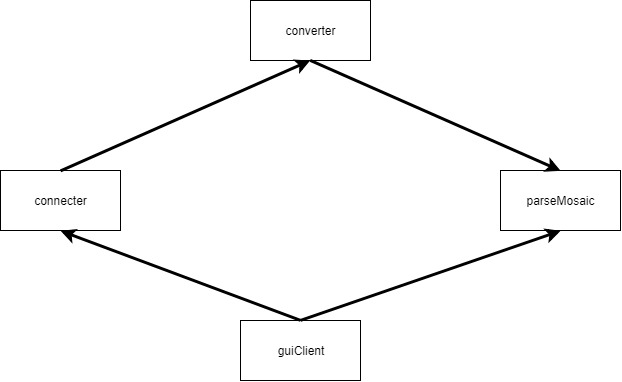
\includegraphics[width=0.7\textwidth]{uh.jpg}
\caption{Use hierarchy among modules}
\label{FigUH}
\end{figure}

\section{Schedule}
Please refer to the link to find the current Gantt Chart:
\color{blue}
\href{https://gitlab.cas.mcmaster.ca/liangw15/3XA3Project/blob/working/ProjectSchedule/Group12_Gantt03.pdf}{ Gantt03}

\color{black}

%\section*{References}

\bibliographystyle {plainnat}
\bibliography {MG}

\end{document}